\section{Reddening and Extinction}

Reddening and extinction are \textit{nearly} the same thing, but not quite. They're both caused by light scattering off dust, but \textit{extinction} describes the dimming that results, and \textit{reddening} describes the preferential scattering of blue light (i.e., more shorter wavelength light gets scattered away from us than longer wavelengths, so we see objects as redder than they actually are.) This is important because it's a pretty large source of systematic uncertainty in supernova studies! Dust doesn't emit light, it just takes it away, so we can't ``see'' it directly. \textit{HOW} are we supposed to correct for an effect we know so little about? 

\subsection{Background}
Extinction, in general, is described by the equation:
\begin{equation}
    A_{V} = -2.5\log \frac{F_{V}}{F_{V,0}},
\end{equation}

where the subscript $V$ indicates the $V$-band photometric bandpass, $F_{V}$ is observed flux in the $V$-band, and $F_{V, 0}$ is the intrinsic flux in the $V$-band.

Reddening is described by:
\begin{equation}
    E(B-V) = (B-V)_{observed} - (B-V)_{intrinsic},
\end{equation}

where $(B-V)_{observed}$ is the observed $B-V$ photometric color, and $(B-V)_{intrinsic}$ is the intrinsic photometric color. Note that because magnitudes are logarithmic, this equation is a ratio, too! We can link extinction and reddening with an equation, as well:
\begin{equation}
    E(B-V) = A_{B} - A_{V},
\end{equation}

where $A_{B}$ is photometric extinction in the $B$-band and $A_{V}$ is photometric extinction in the $V$-band. We can also link them like this:
\begin{equation}
    A_{V} = R_{V}E(B-V),
\end{equation}

where $R_{V}$ is a constant called the ``total-to-selective extinction ratio''. Basically, it's a constant that tells you how much light you lose in a particular photometric band. 

\begin{figure}
    \centering
    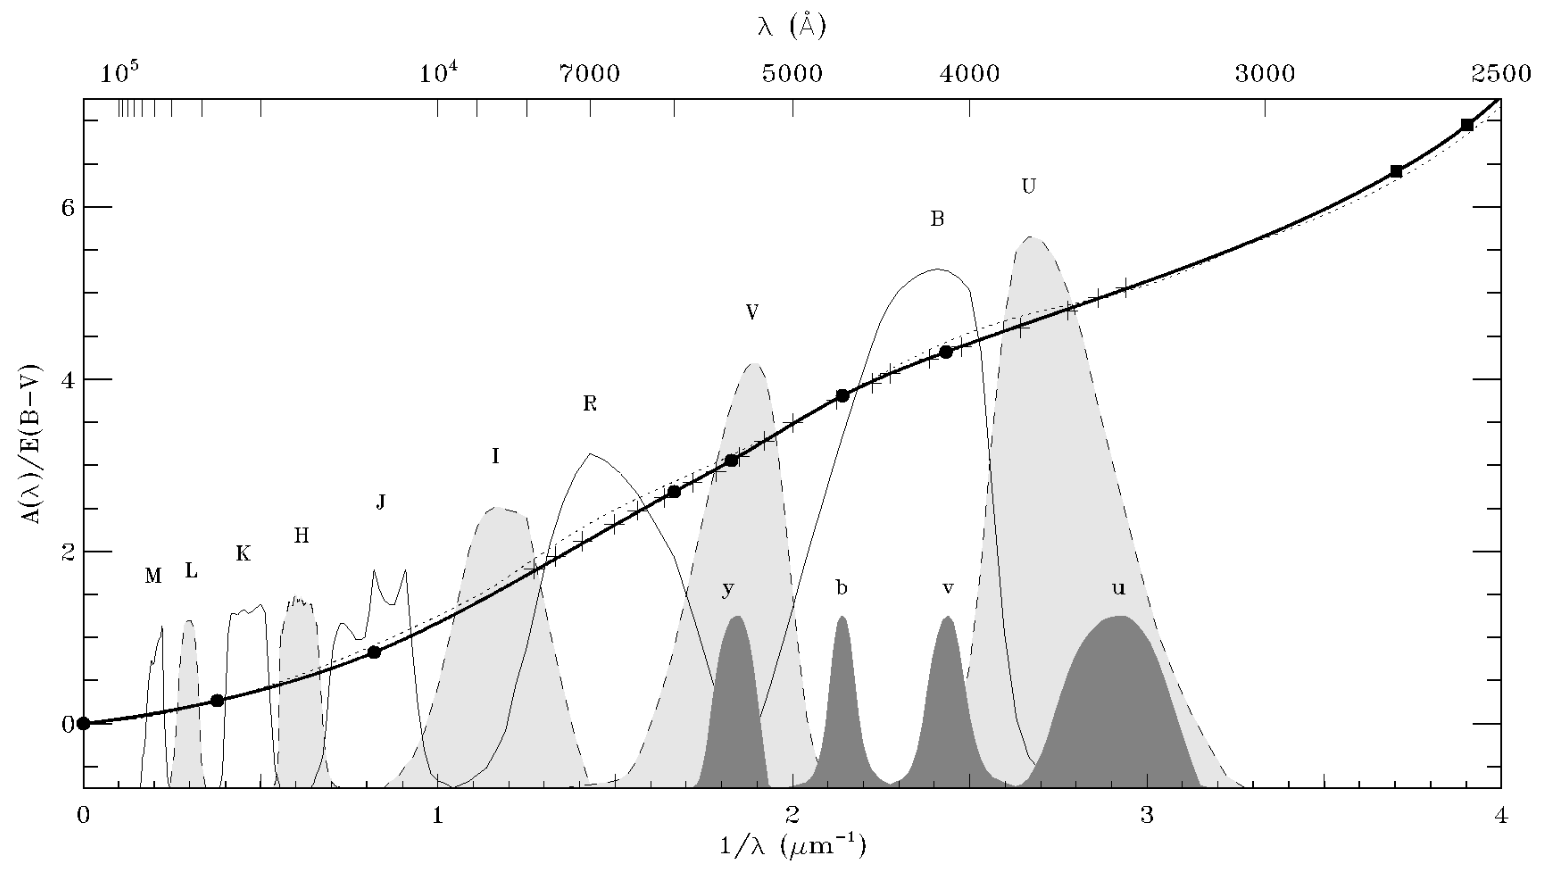
\includegraphics[width=0.99\textwidth]{figs/fitzpatrick1999.png}
    \caption{$R_{X}$ ($X$ for an arbitrary filter) for Johnson photometric filters (transmission functions shown scaled arbitrarily for reference). Solid points are data, the solid line is a cubic spline interpolation (\textit{not} a fit). Note that extinction has a more significant effect at shorter wavelengths. Figure from \cite{Fitzpatrick1999}.}
    \label{fig:phot_reddening}
\end{figure}

\subsection{Correcting for Dust}

There are a few packages you can use to quickly un-dust your data. First, \href{https://dust-extinction.readthedocs.io/en/stable/}{\texttt{dust\_extinction}} has a bunch of dust extinction curves and allows you to redden or deredden the spectrum by multiplying or dividing by the dust model's \texttt{extinguish} attribute, respectively. It also takes care of units for you, so you'll need \href{https://docs.astropy.org/en/stable/units/index.html}{\texttt{astropy}'s \texttt{units} module}. You have to provide it with $E(B-V)$ or $A_{V}$ as well. I like to get that with the SNooPy \texttt{get\_dust\_RADEC()} function, which retrieves the Milky Way $E(B-V)$ from \href{https://irsa.ipac.caltech.edu/frontpage/}{IRSA} based on RA and Dec (Section~\ref{sec:snpydustfuncs}). Here's some pseudocode showing how I deredden the flux for a spectrum:

\begin{minted}[
    bgcolor=lightgray,
    frame=leftline,
    framesep=-3mm]
    {python}

    from astropy import units as u
    from dust_extinction.parameter_averages import F04
    from snpy.utils.IRSA_dust_getval import get_dust_RADEC

    dustmodel = F04(Rv=3.1)
    mwreddening = get_dust_RADEC(ra, dec, calibration='SF11')[0][0]
    dereddened_flux = ((flux*u.erg/(u.s*u.AA*u.cm**2))/
        dustmodel.extinguish(wave*u.AA, Ebv=mwreddening)).value
    
\end{minted}